\section{Data and exploratory analysis}
\label{section:data}

\paragraph{Data.} We use two PhysioNet databases. The MIT-BIH Arrhythmia Database contains 48 half-hour, two-channel ECG recordings from 47 subjects, sampled at 360~Hz, with every beat labelled by cardiologists \cite{moody2001impact}; we use the MLII lead. The MIT-BIH Noise Stress Test Database contains recorded ambulatory noise of three types: baseline wander, muscle artefact and electrode motion \cite{moody1984noise}. Following de Chazal et al.~\cite{dechazal2004automatic}, we split the recordings by patient: 22 recordings for training (DS1) and 22 for testing (DS2), leaving out the four recordings of patients with pacemakers. Records 201 and 202 come from the same subject \cite{moody2001impact}, so we drop 202 from the test set to keep the two groups of patients completely separate. Each beat is cut out from 250~ms before to 450~ms after its R peak, after a 0.5--40~Hz band-pass filter, and labelled with one of the five standard classes N, S, V, F and Q (Table~\ref{tab:classes}).

\begin{table}[H]
\caption{Beats per class in the training and test patients.}
\label{tab:classes}
\centering
\small
\setstretch{1.1}
\begin{tabular}{@{}lrrrrrr@{}}
\toprule
 & \textbf{N} & \textbf{S} & \textbf{V} & \textbf{F} & \textbf{Q} & \textbf{Total} \\
\midrule
Training (DS1, 22 patients) & 45\,824 & 943 & 3\,788 & 414 & 8 & 50\,977 \\
Test (DS2, 21 patients) & 42\,159 & 1\,781 & 3\,200 & 387 & 7 & 47\,534 \\
\bottomrule
\end{tabular}
\end{table}

\paragraph{What the data show.} About 90\% of all beats are normal, so accuracy alone would be misleading and we report results per class. Figure~\ref{fig:beats} shows the average beat of each class: ventricular (V) beats have a wide, deformed QRS complex, while supraventricular (S) beats look almost like normal ones. What distinguishes S beats is their timing: their median preceding RR interval is 82\% of the local average, compared with 73\% for V beats and 100\% for normal beats (Figure~\ref{fig:rr}).

\begin{figure}[H]
\centering
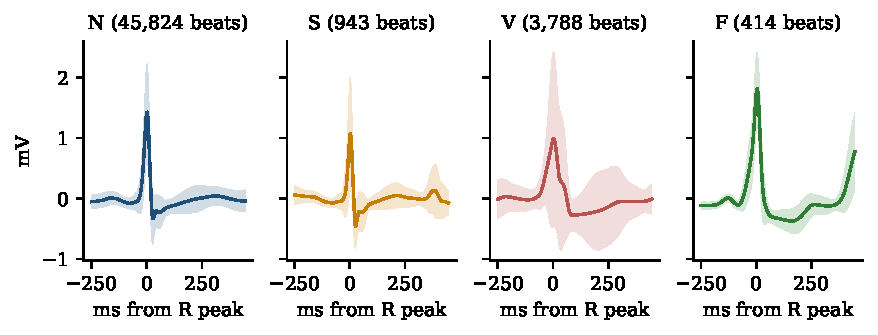
\includegraphics[width=\textwidth]{Fig/s4_eda_beats.pdf}
\caption{Average beat ($\pm$ one standard deviation) of each class in the training patients.}
\label{fig:beats}
\end{figure}

\begin{figure}[H]
\centering
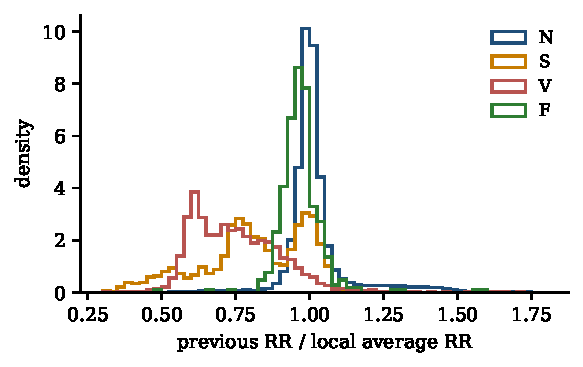
\includegraphics[width=0.65\textwidth]{Fig/s4_eda_rr.pdf}
\caption{Timing of each beat relative to the local rhythm: premature beats (S, V) arrive early.}
\label{fig:rr}
\end{figure}

Figure~\ref{fig:patients} shows why a personal model is useful. Across the 43 patients, a normal beat differs from the same patient's typical beat by 0.058~mV (median RMS), but typical beats of two different patients differ by 0.252~mV, more than four times as much. A model of a normal beat is therefore much more precise when it is built for one patient. Figure~\ref{fig:noise} shows the three noise types we add to test the Signal Monitoring agent.

\begin{figure}[H]
\centering
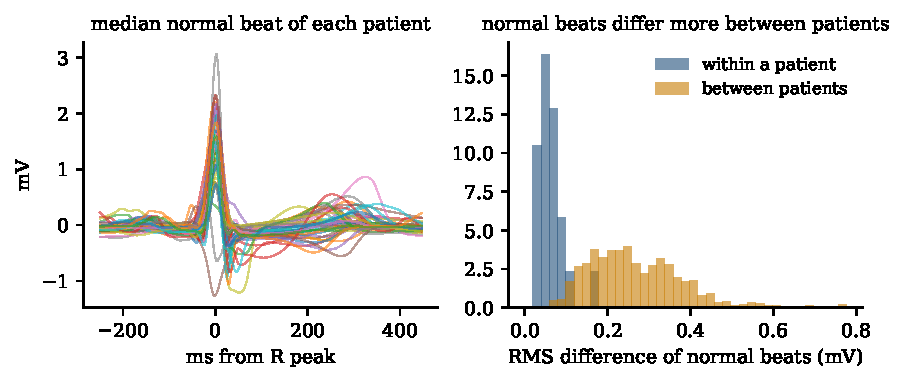
\includegraphics[width=\textwidth]{Fig/s4_eda_patients.pdf}
\caption{Left: the typical normal beat of each of the 43 patients. Right: normal beats vary much less within one patient than between patients.}
\label{fig:patients}
\end{figure}

\begin{figure}[H]
\centering
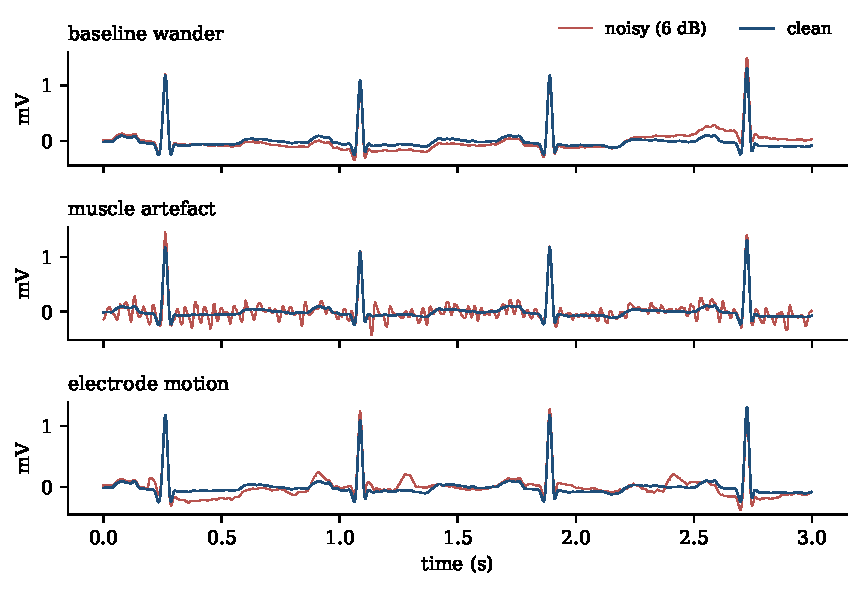
\includegraphics[width=0.75\textwidth]{Fig/s4_eda_noise.pdf}
\caption{A clean ECG segment with each recorded noise type added at a signal-to-noise ratio of 6~dB.}
\label{fig:noise}
\end{figure}
